% =============================================================================
% The Evolution of Information Retrieval: From Sparse to Neural, Hybrid, and
% LLM-Augmented Approaches
% =============================================================================

\documentclass[12pt, a4paper]{article}

% --- Packages ----------------------------------------------------------------
\usepackage[margin=2.5cm]{geometry}
\usepackage{amsmath, amssymb}
\usepackage{booktabs}       % \toprule, \midrule, \bottomrule
\usepackage{multirow}
\usepackage{graphicx}
\graphicspath{{figures/}}
\usepackage[hyphens]{url}
\usepackage{hyperref}
\usepackage{xcolor}
\usepackage{todonotes}      % \todo{} markers
\usepackage{microtype}
\usepackage{natbib}
\usepackage{caption}
\usepackage{subcaption}
\usepackage{algorithm}
\usepackage{algpseudocode}
\usepackage{float}
\usepackage{tikz}
\usetikzlibrary{arrows.meta}

% --- Convenience macros ------------------------------------------------------
\newcommand{\ndcg}{NDCG@10}
\newcommand{\mrr}{MRR@10}
\newcommand{\map}{MAP@100}
\newcommand{\tc}{TREC-COVID}
\newcommand{\fiqa}{FIQA}
\newcommand{\scifact}{SciFact}
\newcommand{\bvec}[1]{\mathbf{#1}}

% =============================================================================
\begin{document}
% =============================================================================

\title{%
  \textbf{The Evolution of Information Retrieval:}\\
  From Sparse to Neural and Hybrid Retrieval Strategies\\[6pt]
  \large A Comparative Empirical Study on BEIR Benchmarks
}
\author{Sai Krishna B \and Ravindra Babu T}
\date{April 2026}

\maketitle

% =============================================================================
\begin{abstract}
% =============================================================================
Information retrieval (IR) has undergone a paradigm shift over the past decade,
moving from hand-crafted statistical methods toward deep neural representations
and hybrid multi-stage pipelines.  This study traces that evolution across four
phases: (1)~classical sparse retrieval (BoW, TF-IDF, BM25); (2)~early neural
retrieval (Word2Vec mean/IDF pooling); (3)~dense bi-encoder retrieval (MiniLM,
MPNet, BGE, E5); (4)~hybrid retrieval with cross-encoder reranking (Reciprocal
Rank Fusion + \texttt{ms-marco-MiniLM-L-6-v2}).  We further investigate
domain-specific fine-tuning of a 22M-parameter encoder using
MultipleNegativesRankingLoss.

All experiments are evaluated on three BEIR benchmarks with distinct
characteristics: \fiqa{} (financial Q\&A, conversational), \scifact{}
(scientific claim verification), and \tc{} (biomedical passage retrieval).
Our results show that BGE-base dominates zero-shot dense retrieval
(\ndcg{}~0.78 on \tc{}); the cross-encoder reranker is a more reliable upgrade
than hybrid RRF when the sparse component is weak: BGE alone (0.781)
outperforms hybrid+reranker (0.763) on \tc{}; and 919-pair domain-specific
fine-tuning yields +7.7\% in-domain NDCG with minimal negative transfer across
other domains.  We identify concrete failure modes at each stage: BM25
length-normalisation degrading on uniform-length corpora, Word2Vec silently
dropping out-of-vocabulary biomedical identifiers, DPR collapsing on
out-of-domain queries, and equal-weight RRF diluting a dominant dense signal.
\end{abstract}

\tableofcontents
\newpage

% =============================================================================
\section{Introduction}
\label{sec:intro}
% =============================================================================

Information retrieval underpins almost every modern NLP application, from
search engines to retrieval-augmented generation (RAG) systems.  Historically,
term-overlap methods such as BM25~\citep{robertson2009probabilistic} dominated
the field, offering strong baselines with no training requirements.  The
introduction of dense embeddings via BERT~\citep{devlin2019bert} and the
Sentence-BERT (SBERT) bi-encoder framework~\citep{reimers2019sentence} opened
a new era where semantic similarity could be computed in a continuous vector
space, enabling retrieval of relevant documents even when query and passage
share no lexical overlap.  SBERT established the Siamese bi-encoder
architecture that all subsequent dense retrievers build upon; this study
evaluates its successors (MiniLM, MPNet, BGE, E5) rather than the
original model.

More recently, instruction-tuned embedding models such as
BGE~\citep{xiao2023c} and E5~\citep{wang2022text} have pushed the frontier
further, while hybrid pipelines that fuse sparse and dense signals via
Reciprocal Rank Fusion (RRF)~\citep{cormack2009reciprocal} followed by
cross-encoder reranking have become the de-facto production architecture.
Simultaneously, large language models (LLMs) are increasingly used as
\emph{judges} to evaluate retrieval quality beyond the limitations of
manually annotated relevance judgements (qrels).

\paragraph{Contributions.}
\begin{enumerate}
  \item A systematic, reproducible comparison of four IR paradigms on three
        heterogeneous BEIR benchmarks using unified evaluation metrics.
  \item Identification of concrete failure modes at each stage: BM25
        length-normalisation degrading on uniform-length corpora (\scifact{},
        \fiqa{}); Word2Vec silently dropping OOV biomedical identifiers;
        DPR collapsing out-of-domain; equal-weight RRF diluting a dominant
        dense signal when the sparse component is weak.
  \item Per-query working and failure examples for each method, making
        failure modes tangible rather than aggregate.
  \item Empirical evidence that 919-pair domain fine-tuning with
        MultipleNegativesRankingLoss yields competitive gains, and that
        combined multi-domain training generalises to unseen domains
        without negative transfer.
\end{enumerate}

% =============================================================================
\section{Background}
\label{sec:background}
% =============================================================================

\subsection{Evaluation Benchmarks}
\label{sec:benchmarks}

We evaluate on three BEIR~\citep{thakur2021beir} datasets spanning diverse
retrieval domains and query types.  Table~\ref{tab:datasets} summarises the
key statistics.

\begin{table}[h]
\centering
\caption{BEIR benchmark datasets used in this study.}
\label{tab:datasets}
\resizebox{\textwidth}{!}{%
\begin{tabular}{lllrrll}
\toprule
\textbf{Dataset} & \textbf{Domain} & \textbf{Task} & \textbf{Corpus} & \textbf{Test queries} & \textbf{Relevance} & \textbf{Avg.\ words/passage} \\
\midrule
\fiqa{}    & Financial Q\&A    & Answer retrieval    & 57,638  & 648 & Binary (0/1)   & 133 \\
\scifact{} & Scientific claims & Claim verification  & 5,183   & 300 & Binary (0/1)   & 215 \\
\tc{}      & Biomedical        & Passage retrieval   & 171,332 & 50  & Graded (0/1/2) & 161 \\
\bottomrule
\end{tabular}
}
\end{table}

\begin{description}
  \item[\fiqa{}]  648 financial community Q\&A questions; 57,638 passages.
        Queries are informal, conversational, and domain-specific (sourced from
        Reddit and StackExchange).  Relevance labels in the original FiQA
        challenge were graded; the BEIR test split binarises all qrels to
        score~$=1$.  BM25 is well-known to underperform on conversational queries.
  \item[\scifact{}]  300 scientific claim queries; 5,183 abstracts.  Relevance
        requires domain understanding; exact-term matching often fails on
        paraphrase-style claims.  On average only 1.1 relevant passages exist
        per query, making Recall@10 a demanding metric.
  \item[\tc{}]  50 COVID-19 biomedical questions; 171,332 PubMed abstracts.
        Relevance is graded: 0 (not relevant), 1 (partially), 2 (highly).
        With 493 relevant passages per query on average, Recall@100 captures
        only $\sim$12\% of all relevant documents (a corpus-coverage limit,
        not a model limit).
\end{description}

\paragraph{Example queries and passages.}
To illustrate the diversity of query styles across datasets:

\begin{itemize}
  \item \textbf{\fiqa{}}: \textit{``How should I invest my first \$1{,}000?''} \\
        \textit{Relevant passage:} ``For small amounts, low-cost index funds
        tracking the S\&P 500 provide broad diversification with minimal fees.
        Consider a Roth IRA if you have earned income\ldots''

  \item \textbf{\scifact{}}: \textit{``Headaches are not correlated with
        cognitive impairment.''} \\
        \textit{Relevant passage:} ``Analysis of 412 patients found no
        significant association between cephalgia frequency and neurocognitive
        function scores (p\,=\,0.43), after adjusting for age and comorbidities.''

  \item \textbf{\tc{}}: \textit{``What are the symptoms of COVID-19?''}
        (graded relevance; same query, three passages at different relevance levels)
        \begin{itemize}
          \item \textbf{Grade~2 (highly relevant):}
                ``Common manifestations include fever, dry cough, and fatigue.
                Less common symptoms are myalgia, sore throat, diarrhoea,
                conjunctivitis, and headache.  Dyspnoea occurs in severe cases.''
          \item \textbf{Grade~1 (partially relevant):}
                ``Coronavirus infections generally present with respiratory
                symptoms; some patients remain asymptomatic with detectable
                viral load, complicating containment.''
          \item \textbf{Grade~0 (not relevant):}
                ``Influenza vaccination rates among healthcare workers declined
                during the 2019--20 season due to temporary supply shortages
                at regional distribution centres.''
        \end{itemize}
\end{itemize}

\paragraph{Metric validity on graded relevance (\tc{}).}
\tc{} uses graded relevance (0, 1, 2), while \fiqa{} and \scifact{} use
binary labels.  NDCG@10 handles graded relevance natively via
$\text{rel}_i / \log_2(i+1)$ and is the primary metric throughout this
study.  MRR and Recall, however, binarise at grade~$\geq 1$: MRR treats
a partially relevant (grade~1) hit identically to a highly relevant
(grade~2) hit, and Recall@$k$ counts all grade-$\geq 1$ documents as the
relevant set, which includes 493 passages per query on average in \tc{}.
These two effects make MRR and Recall less informative for \tc{} than
for the other two datasets; NDCG@10 should be the basis for any
cross-dataset comparison involving \tc{}.

Note the vocabulary gap in the \scifact{} example: the query uses ``headaches''
while the passage uses ``cephalgia''.  Lexical methods score zero; vector-based
methods can bridge this gap when the words are nearby in embedding space.

% -----------------------------------------------------------------------------
\subsection{Evaluation Metrics}
\label{sec:metrics}
% -----------------------------------------------------------------------------

Following BEIR convention we report the metrics below.  All metrics are
averaged over queries.

\paragraph{NDCG@10 (Normalised Discounted Cumulative Gain).}
Primary ranking quality metric.  Rewards retrieving relevant documents early
in the ranking.
\begin{equation}
  \text{DCG@}k = \sum_{i=1}^{k} \frac{\text{rel}_i}{\log_2(i+1)}, \qquad
  \text{NDCG@}k = \frac{\text{DCG@}k}{\text{IDCG@}k}
  \label{eq:ndcg}
\end{equation}
where $\text{rel}_i \in \{0,1,2\}$ is the relevance of the document at rank
$i$, and IDCG@$k$ is the ideal (best-possible) DCG@$k$.

\paragraph{MRR@10 (Mean Reciprocal Rank).}
Measures how quickly the first relevant document is found.
\begin{equation}
  \text{MRR@}k = \frac{1}{|Q|} \sum_{q \in Q}
    \frac{1}{\text{rank}_{q}^{\text{first relevant}}}
  \label{eq:mrr}
\end{equation}
The retrieved list is truncated to top-$k$ \emph{before} passing to
\texttt{pytrec\_eval}, preventing rank-cutoff inflation on weaker models.

\paragraph{MAP@100 (Mean Average Precision).}
\begin{equation}
  \text{MAP@100} = \frac{1}{|Q|} \sum_{q \in Q} \text{AP}_q, \qquad
  \text{AP}_q = \frac{1}{R_q} \sum_{k=1}^{100} P@k \cdot \mathbb{1}[\text{doc}_k\text{ relevant}]
  \label{eq:map}
\end{equation}
where $R_q$ is the total number of relevant documents for query $q$, and $P@k$
is precision at rank $k$.

\paragraph{Recall@$k$.}
\begin{equation}
  \text{Recall@}k = \frac{|\text{Rel} \cap \text{Retrieved@}k|}{|\text{Rel}|}
  \label{eq:recall}
\end{equation}
Reported at $k \in \{10, 50, 100\}$.  On \tc{}, Recall@100 is inherently low
($\sim$0.12) due to the large number of relevant documents per query.

% -----------------------------------------------------------------------------
\subsection{Reciprocal Rank Fusion}
\label{sec:rrf}
% -----------------------------------------------------------------------------

Given ranked lists $L_1, \ldots, L_n$ from $n$ retrievers, the RRF score for
document $d$ is:
\begin{equation}
  \text{RRF}(d) = \sum_{i=1}^{n} \frac{1}{k + \text{rank}_i(d)}
  \label{eq:rrf}
\end{equation}
where $k = 60$ (standard default) smooths the contribution of documents ranked
low in one list but high in another, preventing a single high-rank appearance
from dominating the fusion.  We fuse BM25 and BGE ranked lists.

% -----------------------------------------------------------------------------
\subsection{Training Loss Functions}
\label{sec:losses}
% -----------------------------------------------------------------------------

Three loss functions are widely used for training dense retrievers.

\paragraph{Contrastive Loss~\citep{hadsell2006dimensionality}.}
The earliest metric-learning loss.  Given a labelled pair $(x_i, x_j)$ with
label $y \in \{0, 1\}$ (1 = similar, 0 = dissimilar) and distance
$d = \|f(x_i) - f(x_j)\|$:
\begin{equation}
  \mathcal{L}_{\text{contrastive}} = y \cdot d^2
    + (1 - y) \cdot \max(0,\, m - d)^2
  \label{eq:contrastive}
\end{equation}
where $m > 0$ is a margin.  Requires explicit pair labels; does not scale
well to large corpora.

\paragraph{Triplet Loss~\citep{schroff2015facenet}.}
Trains on (query, positive, negative) triplets.  Used in the original SBERT:
\begin{equation}
  \mathcal{L}_{\text{triplet}} = \max\!\bigl(0,\;
    d(q, p^+) - d(q, p^-) + m \bigr)
  \label{eq:triplet}
\end{equation}
where $d$ is a distance function (e.g.\ cosine or Euclidean), $p^+$ is a
relevant passage, $p^-$ is a hard negative, and $m$ is the margin (typically
0.5--1.0).  Requires explicit hard-negative mining.

\paragraph{MultipleNegativesRankingLoss (MNR / InfoNCE).}
Current best practice for bi-encoder training~\citep{henderson2017efficient}:
\begin{equation}
  \mathcal{L}_{\text{MNR}} = -\frac{1}{B} \sum_{i=1}^{B}
    \log \frac{e^{\,\text{sim}(\bvec{q}_i,\,\bvec{p}_i) / \tau}}
              {\displaystyle\sum_{j=1}^{B}
               e^{\,\text{sim}(\bvec{q}_i,\,\bvec{p}_j) / \tau}}
  \label{eq:mnr}
\end{equation}
where $B$ is the batch size, $(\bvec{q}_i, \bvec{p}_i)$ is the $i$-th
(query, positive passage) pair, and $\tau$ is the temperature.  All other
positives in the batch act as \emph{in-batch negatives}; no hard-negative
mining is required.  We use MNR in this study because BEIR qrels directly
supply (query, positive) pairs and batch mates are free negatives.

\begin{table}[h]
\centering
\caption{Comparison of bi-encoder training losses.}
\label{tab:losses}
\begin{tabular}{llll}
\toprule
\textbf{Loss} & \textbf{Negatives} & \textbf{Scalability} & \textbf{Notes} \\
\midrule
Contrastive & Explicit labelled pairs & Low    & Early metric learning \\
Triplet     & Hard-mined triplets      & Medium & SBERT v1; needs mining \\
MNR/InfoNCE & In-batch (free)          & High   & Current best practice \\
\bottomrule
\end{tabular}
\end{table}

% =============================================================================
\section{Experimental Setup}
\label{sec:setup}
% =============================================================================

\begin{description}
  \item[Hardware]  Apple M5 (15-core CPU, 16-core GPU, 24\,GB unified memory).
        PyTorch MPS backend; FAISS replaced with exact numpy dot-product search
        to avoid OpenMP library conflicts on macOS (\texttt{libomp} conflict
        \#15 / SIGABRT).
  \item[Software]  Python~3.12; \texttt{sentence-transformers~5.4.1};
        \texttt{transformers~4.x}; \texttt{torch~2.x} (MPS backend);
        \texttt{gensim~4.x} (Word2Vec); \texttt{scikit-learn} (TF-IDF/BoW);
        \texttt{rank-bm25}; \texttt{beir}; \texttt{pytrec\_eval}.
  \item[Replication]  All scripts in \texttt{scripts/}; results persisted to
        \texttt{results/} as JSON; notebooks in \texttt{notebooks/} reproduce
        all plots and tables.
\end{description}

% =============================================================================
\section{Phase 1: Sparse Retrieval}
\label{sec:sparse}
% =============================================================================

% -----------------------------------------------------------------------------
\subsection{Methods}
% -----------------------------------------------------------------------------

\subsubsection*{Bag-of-Words (BoW)}

Each document is represented as a vector of raw term counts over the corpus
vocabulary $V$.  Query--document similarity is cosine similarity over count
vectors:
\begin{equation}
  \text{score}_{\text{BoW}}(q, d) = \cos(\mathbf{v}_q,\, \mathbf{v}_d),
  \quad \mathbf{v}_d[t] = \text{tf}(t, d)
  \label{eq:bow}
\end{equation}
where $\text{tf}(t, d)$ is the \textbf{term frequency}, i.e., the raw count of
how many times term $t$ appears in document $d$.
\textbf{Limitation:} high-frequency stop words (``the'', ``is'', ``a'')
dominate the dot product and dilute discriminative signal.

\subsubsection*{TF-IDF}

Weights each term by its \emph{inverse document frequency}, down-weighting
common words and up-weighting rare, discriminative ones:
\begin{equation}
  w(t, d) = \text{tf}(t, d) \times \text{idf}(t), \quad
  \text{idf}(t) = \log\!\frac{N}{\text{df}(t)}
  \label{eq:tfidf}
\end{equation}
\begin{equation}
  \text{score}_{\text{TF-IDF}}(q, d) = \cos(\mathbf{w}_q,\, \mathbf{w}_d)
  \label{eq:tfidf_score}
\end{equation}
where $N$ is the corpus size and $\text{df}(t)$ is the number of documents
containing term $t$.  In practice, scikit-learn applies sublinear TF scaling
($\text{tf} \leftarrow 1 + \log \text{tf}$), dampening the effect of
high-frequency terms.  The cosine similarity implicitly L2-normalises document
vectors, providing a soft global length normalisation.

\subsubsection*{BM25 (Best Match 25)}

BM25, introduced in the early 1990s~\citep{robertson1994simple} and
formally surveyed in~\citet{robertson2009probabilistic}, adds two important
corrections over TF-IDF:

\begin{equation}
  \text{score}_{\text{BM25}}(q, d)
    = \sum_{t \in q} \text{IDF}(t)
      \cdot \frac{f(t,d) \cdot (k_1 + 1)}
                 {f(t,d) + k_1 \!\left(1 - b + b\,\dfrac{|d|}{\text{avgdl}}\right)}
  \label{eq:bm25}
\end{equation}
\begin{equation}
  \text{IDF}(t) = \log\!\left(\frac{N - \text{df}(t) + 0.5}{\text{df}(t) + 0.5} + 1\right)
  \label{eq:bm25_idf}
\end{equation}

\noindent\textbf{Parameters:}
\begin{itemize}
  \item $f(t, d)$: term frequency of term $t$ in document $d$ (identical to
        $\text{tf}(t,d)$ in Eq.~\ref{eq:bow}).  The saturation formula in the
        numerator/denominator replaces the raw count used in TF-IDF.
  \item $k_1 \in [1.2,\, 2.0]$: \emph{term-frequency saturation}:
        controls how much weight additional occurrences of a term add.
        At $k_1 = 0$ all occurrences beyond the first are ignored;
        as $k_1 \to \infty$ the score approaches raw TF.  Default: 1.5.
  \item $b \in [0,\, 1]$: \emph{length normalisation strength}:
        $b = 0$ disables length penalty, $b = 1$ fully normalises by document
        length.  Default: 0.75 (calibrated on MS MARCO and similar long-document
        collections).
  \item $|d|$: document length in terms; $\text{avgdl}$: corpus-average length.
\end{itemize}

% -----------------------------------------------------------------------------
\subsection{Experimental Results}
% -----------------------------------------------------------------------------

\begin{table}[h]
\centering
\caption{Sparse retrieval: \ndcg{} across all datasets.}
\label{tab:sparse}
\begin{tabular}{lccc}
\toprule
\textbf{Method} & \textbf{\tc{}} & \textbf{\fiqa{}} & \textbf{\scifact{}} \\
\midrule
BoW             & 0.1763 & 0.0656 & 0.3647 \\
TF-IDF          & 0.2866 & \textbf{0.1793} & \textbf{0.6286} \\
BM25            & \textbf{0.4471} & 0.1591 & 0.5597 \\
\bottomrule
\end{tabular}
\end{table}

\paragraph{Findings.}
BM25 is the best sparse method on \tc{}, but TF-IDF beats BM25 on \fiqa{}
and \scifact{}.  The gap on \tc{} (0.287 vs.\ 0.447) illustrates BM25's
length-normalisation advantage on long biomedical abstracts (mean 161 words,
high variance).  The TF-IDF inversion on \fiqa{} and \scifact{} is
\emph{structural}, not a hyperparameter issue, as detailed in
Section~\ref{sec:bm25_sweep} below.

\paragraph{Illustrative per-query examples.}
\begin{itemize}

\item \textbf{BoW worked.}\\
  \textit{Query:} ``AIRE is expressed in some skin tumors.'' (\scifact{})\\
  \textit{Expected passage:} \textit{Keratin-dependent regulation of Aire and gene expression
    in skin tumor keratinocytes.} ``Expression of K17 is robustly upregulated in tumors
    originating in stratified epithelia; Aire is inducibly expressed in human and mouse
    tumor keratinocytes.''\\
  \textit{Why it worked:} Three rare tokens (\texttt{AIRE}, \texttt{skin}, \texttt{tumors})
    appear verbatim in the passage; their high cosine contribution puts the relevant passage
    at rank~1 despite no stop-word suppression.

\item \textbf{BoW failed (zero vocabulary overlap).}\\
  \textit{Query:} ``0-dimensional biomaterials show inductive properties.'' (\scifact{})\\
  \textit{Expected passage:} \textit{New opportunities: the use of nanotechnologies to
    manipulate and track stem cells.} ``Examples include magnetic nanoparticles and quantum
    dots for stem cell labeling and in vivo tracking.''\\
  \textit{Retrieved (rank 1):} \textit{US28 chemokine receptor constitutive endocytosis.}
    ``US28 is one of four transmembrane chemokine receptors encoded by human
    cytomegalovirus.''\\
  \textit{Why it failed:} No token in the query (\texttt{0-dimensional}, \texttt{biomaterials},
    \texttt{inductive}) overlaps with any token in the relevant passage (\texttt{nanotechnologies},
    \texttt{quantum}, \texttt{dots}); cosine similarity is zero and stop words push a
    completely unrelated CMV passage to rank~1.

\item \textbf{TF-IDF won where BoW failed.}\\
  \textit{Query:} ``ADAR1 binds to Dicer to cleave pre-miRNA.'' (\scifact{})\\
  \textit{Expected passage:} \textit{ADAR1 Forms a Complex with Dicer to Promote MicroRNA
    Processing.} ``ADAR1 forms a complex with Dicer through direct protein-protein
    interaction and increases the maximum rate of pre-miRNA cleavage by Dicer.''\\
  \textit{BoW rank-1 (wrong):} \textit{Phosphate and R2D2 restrict the substrate specificity
    of Dicer-2.} ``Drosophila Dicer-2 generates siRNAs from long double-stranded RNA; Dicer-1
    produces miRNAs from pre-miRNA.'' (\texttt{Dicer} matches, but \texttt{ADAR1} is absent)\\
  \textit{Why TF-IDF won:} \texttt{ADAR1} is rare across the corpus and carries very high
    IDF; TF-IDF amplifies its weight to lift the correct passage to rank~1.  BoW treats
    \texttt{Dicer} and \texttt{ADAR1} as equally weighted and retrieves a Dicer-only passage.

\item \textbf{All sparse methods failed (surface overlap cannot resolve claim specificity).}\\
  \textit{Query:} ``A deficiency of vitamin B12 increases blood levels of homocysteine.'' (\scifact{})\\
  \textit{Expected passage:} \textit{Randomized trial of folic acid supplementation and serum
    homocysteine levels.} ``Lowering serum homocysteine with folic acid is expected to reduce
    mortality from ischemic heart disease; homocysteine reduction is maximal at 1\,mg/d folic
    acid.''\\
  \textit{Retrieved (rank 1, all three methods):} BoW, TF-IDF, and BM25 each retrieve a
    different passage from the same metabolic topic area, but none retrieves the annotated
    relevant passage at rank~1.  For example, BM25 returns: \textit{Folate status and plasma
    homocysteine response to supplementation.} ``High plasma total homocysteine (tHcy) is a
    risk factor for vascular diseases; we investigated the extent to which serum folate and
    plasma tHcy respond to supplementation.''\\
  \textit{Why all failed:} The query, the expected passage, and the retrieved passages all
    share surface tokens (\texttt{homocysteine}, \texttt{vitamin}, \texttt{blood},
    \texttt{levels}, \texttt{deficiency}, \texttt{folate}).  No lexical method, regardless
    of weighting scheme or length normalisation, can distinguish which passage
    corroborates the specific B12$\to$homocysteine causal claim versus discussing the same
    metabolic pathway from a different angle.  This is a structural limit of surface-form
    matching, not a tuning issue.

\end{itemize}

% -----------------------------------------------------------------------------
\subsection{BM25 Hyperparameter Sweep}
\label{sec:bm25_sweep}
% -----------------------------------------------------------------------------

To investigate why TF-IDF beats BM25 on \scifact{} and \fiqa{}, we sweep
the length-normalisation parameter $b$ and the saturation parameter $k_1$.
Table~\ref{tab:bm25_passage_stats} shows corpus passage-length statistics.

\begin{table}[h]
\centering
\caption{Passage-length statistics per dataset (words).  CV = coefficient of
  variation ($\sigma / \mu$): a dimensionless measure of length dispersion.
  Higher CV indicates more variable passage lengths, making length
  normalisation more important.}
\label{tab:bm25_passage_stats}
\begin{tabular}{lrrrrr}
\toprule
\textbf{Dataset} & \textbf{Count} & \textbf{Mean} & \textbf{Median} & \textbf{Std} & \textbf{CV} \\
\midrule
\scifact{} & 5,183   & 214.6 & 204.0 & 87.3  & 0.41 \\
\fiqa{}    & 57,638  & 132.9 & 90.0  & 128.7 & 0.97 \\
\tc{}      & 171,332 & 161.2 & 168.0 & 135.0 & 0.84 \\
\bottomrule
\end{tabular}
\end{table}

\begin{table}[h]
\centering
\caption{$b$ sweep ($k_1=1.5$ fixed): \ndcg{}.  Bold = best BM25 per dataset.
  TF-IDF column for reference.}
\label{tab:bm25_b_sweep}
\begin{tabular}{lrrrrrl}
\toprule
\textbf{Dataset} & $b=0.0$ & $b=0.25$ & $b=0.5$ & $b=0.75$ & $b=1.0$ & \textbf{TF-IDF} \\
\midrule
\scifact{}  & 0.547 & 0.558 & 0.556 & 0.560 & \textbf{0.563} & \textbf{0.629} \\
\fiqa{}     & 0.099 & 0.147 & \textbf{0.162} & 0.159 & 0.039 & \textbf{0.179} \\
\tc{}       & 0.337 & 0.460 & \textbf{0.479} & 0.447 & 0.317 & 0.287 \\
\bottomrule
\end{tabular}
\end{table}

\begin{table}[h]
\centering
\caption{$k_1$ sweep ($b=0.75$ fixed): \ndcg{}.  Bold = best BM25 per dataset.}
\label{tab:bm25_k1_sweep}
\begin{tabular}{lrrrrr}
\toprule
\textbf{Dataset} & $k_1=0.5$ & $k_1=1.0$ & $k_1=1.5$ & $k_1=2.0$ & $k_1=2.5$ \\
\midrule
\scifact{}  & 0.559 & 0.563 & 0.560 & 0.562 & \textbf{0.567} \\
\fiqa{}     & 0.162 & \textbf{0.163} & 0.159 & 0.156 & 0.151 \\
\tc{}       & 0.424 & 0.437 & \textbf{0.447} & 0.438 & 0.441 \\
\bottomrule
\end{tabular}
\end{table}

\paragraph{Interpretation.}
The TF-IDF advantage on \scifact{} and \fiqa{} is \emph{structural}: even
setting $b = 0$ (completely disabling length normalisation) does not close
the gap.  The root cause is that TF-IDF's cosine similarity provides a
\emph{global, implicit} L2 normalisation that outperforms BM25's
\emph{explicit, per-term} length formula on short, relatively uniform
passages.  BM25's $b$ parameter was calibrated on MS MARCO (long, highly
variable documents); it does not transfer well to \scifact{} (CV~0.41)
or \fiqa{}.  The best BM25 on \tc{} is $b=0.5$, confirming that the
default $b=0.75$ over-normalises medium-length biomedical abstracts.

% =============================================================================
\section{Phase 2: Early Neural Retrieval}
\label{sec:early_neural}
% =============================================================================

% -----------------------------------------------------------------------------
\subsection{Word2Vec Architecture}
% -----------------------------------------------------------------------------

Word2Vec~\citep{mikolov2013distributed} trains a shallow neural network
on a large text corpus (Google News, $\sim$100B words) to produce
300-dimensional word vectors.  Two complementary architectures are used:

\begin{itemize}
  \item \textbf{Skip-gram:} Given a centre word $w_t$, predict the
        surrounding context words $w_{t+j}$ within a window of size $W$.
        Objective: maximise $\sum_{j \neq 0,\,|j| \leq W} \log P(w_{t+j} \mid w_t)$.
        Better at representing rare words; used for the Google News vectors.
  \item \textbf{CBOW (Continuous Bag-of-Words):} Given the surrounding
        context words, predict the centre word.  Faster to train; slightly
        weaker on rare vocabulary.
\end{itemize}

\begin{figure}[H]
\centering
\begin{subfigure}[b]{\textwidth}
  \centering
  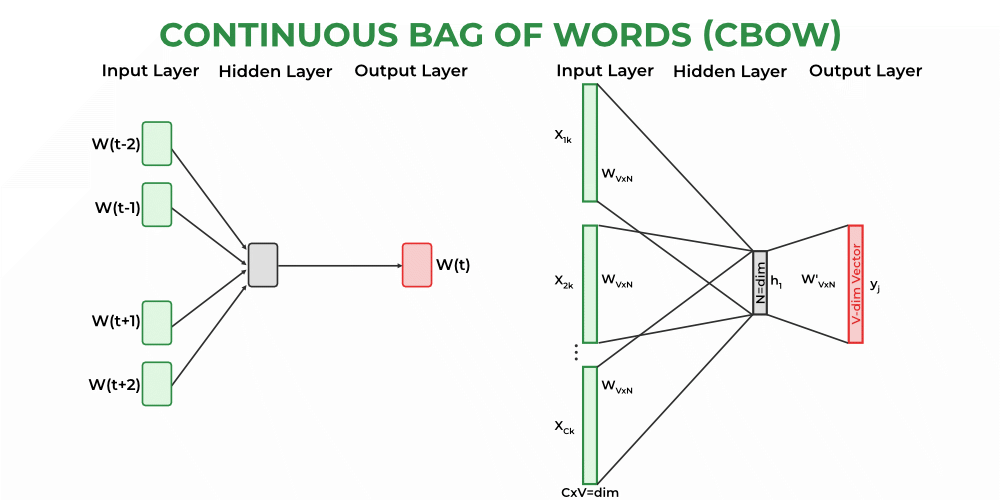
\includegraphics[width=0.78\textwidth]{fig_word2vec_cbow_gfg_rgb.png}
  \caption{CBOW: context words (input) $\to$ centre word (predicted).}
  \label{fig:word2vec_cbow}
\end{subfigure}

\vspace{0.8em}

\begin{subfigure}[b]{\textwidth}
  \centering
  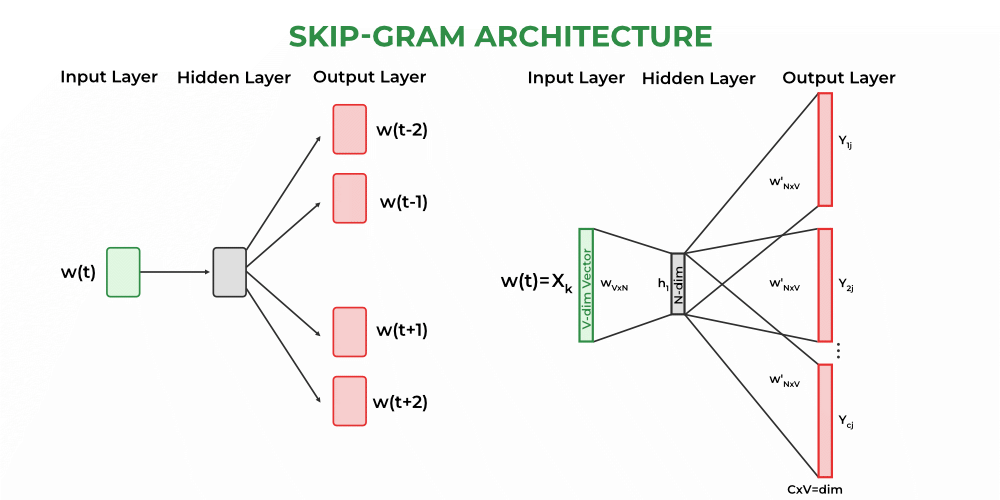
\includegraphics[width=0.78\textwidth]{fig_word2vec_skipgram_gfg_rgb.png}
  \caption{Skip-gram: centre word (input) $\to$ surrounding context words (predicted).}
  \label{fig:word2vec_sg}
\end{subfigure}
\caption{Word2Vec architectures.  CBOW averages context embeddings to predict
  the centre word; Skip-gram inverts this task, predicting all context words
  from the centre word.  Skip-gram is slower but learns better representations
  for rare vocabulary; the Google News checkpoint uses Skip-gram.
  Source: GeeksForGeeks~(\url{https://www.geeksforgeeks.org/nlp/word-embeddings-in-nlp-comparison-between-cbow-and-skip-gram-models/});
  architecture from \citet{mikolov2013distributed}.}
\label{fig:word2vec}
\end{figure}

After training, semantically similar words cluster nearby in the 300-d space:
$\text{vec}(\text{king}) - \text{vec}(\text{man}) + \text{vec}(\text{woman})
\approx \text{vec}(\text{queen})$.

\paragraph{Polysemy collapse.}
A key limitation: every word has exactly one vector regardless of context.
The word ``bank'' receives the same vector whether used in a financial query
(``savings bank'') or a geographical one (``river bank'').  This is a
fundamental flaw for retrieval, where the same surface form may match
irrelevant passages.

\paragraph{GloVe: Global Vectors~\citep{pennington2014glove}.}
Published the same year as Word2Vec, GloVe (Global Vectors for Word
Representation) takes a different training objective but produces similar
300-d static word vectors.  Rather than predicting neighbouring words from
a centre word (a \emph{local} task); GloVe factorises the global
word--word co-occurrence matrix built from the entire corpus:
\begin{equation}
  J = \sum_{i,j=1}^{V} f(X_{ij})
      \bigl(\bvec{w}_i^\top \tilde{\bvec{w}}_j + b_i + \tilde{b}_j
            - \log X_{ij}\bigr)^2
  \label{eq:glove}
\end{equation}
where $X_{ij}$ is the co-occurrence count of words $i$ and $j$, $f(\cdot)$
is a weighting function that down-weights very frequent pairs, and
$\bvec{w}_i, \tilde{\bvec{w}}_j$ are the word and context vectors being
learned.  The intuition is that the \emph{ratio} of co-occurrence
probabilities carries meaning: $P(\text{ice}|\text{solid}) /
P(\text{steam}|\text{solid}) \gg 1$, differentiating ``solid'' from
related but distinct concepts.

\begin{table}[h]
\centering
\caption{Word2Vec vs.\ GloVe: key differences.}
\label{tab:w2v_vs_glove}
\begin{tabular}{lll}
\toprule
\textbf{Property} & \textbf{Word2Vec (Skip-gram)} & \textbf{GloVe} \\
\midrule
Training signal  & Local window prediction & Global co-occurrence matrix \\
Objective        & Cross-entropy (negative sampling) & Weighted least squares \\
Corpus statistics & Implicit, sampled & Explicit, precomputed \\
Typical dim.     & 300 & 50, 100, 200, 300 \\
Common checkpoint & Google News (100B words) & Wikipedia + Gigaword (6B) \\
Analogy tasks    & Comparable & Slightly stronger \\
\bottomrule
\end{tabular}
\end{table}

In practice, GloVe and Word2Vec perform comparably on most IR benchmarks;
the choice between them is usually driven by the available pre-trained
checkpoint rather than any intrinsic superiority.  Both share the same
fundamental limitation: \textbf{static, context-independent representations}
that cannot resolve polysemy.  Our experiments use the Google News Word2Vec
checkpoint; GloVe is presented here as the natural complement and to complete
the picture of the static-embedding era before contextual models.

\paragraph{Related static-embedding variants (not evaluated, shortlisted).}
Several extensions address known Word2Vec limitations and are shortlisted for
future experimentation:
\begin{itemize}
  \item \textbf{FastText}~\citep{bojanowski2017enriching}: represents each word
        as a sum of character $n$-gram vectors, eliminating OOV entirely.
        Terms like \texttt{PCNA} or \texttt{cSMAC}, absent from Google News,
        are decomposed into subword pieces, giving non-zero vectors.
        Drop-in replacement for Word2Vec in the pooling pipeline.
  \item \textbf{Doc2Vec / Paragraph Vectors}~\citep{le2014distributed}: trains
        a dedicated document-level vector $\bvec{d}_i \in \mathbb{R}^{300}$
        alongside word vectors.  Two variants: PV-DM (document ID as an extra
        context slot) and PV-DBOW (document ID predicts sampled words).
        Unlike pooling, the document vector is a \emph{trained} parameter;
        it captures passage-level semantics without the long-passage centroid
        collapse that hurts mean and IDF-weighted pooling on FIQA and SciFact.
        PV-DBOW is shortlisted as the primary experiment; implementation
        planned in \texttt{scripts/run\_doc2vec\_eval.py}.
\end{itemize}

% -----------------------------------------------------------------------------
\subsection{Methods: Pooling Strategies}
% -----------------------------------------------------------------------------

Both aggregation strategies represent a passage as a single vector by
combining its token vectors.

\paragraph{Mean Pooling.}
Uniform average over all token vectors in the passage:
\begin{equation}
  \bvec{d}_{\text{mean}} = \frac{1}{|T|} \sum_{t \in T} \bvec{v}_t
  \label{eq:mean_pool}
\end{equation}
where $T$ is the sequence of tokens and $\bvec{v}_t \in \mathbb{R}^{300}$
is the Word2Vec vector for token $t$.  Equal weight is given to all tokens,
including stop words, which dilutes the semantic signal.

\paragraph{IDF-Weighted Pooling.}
Weights each token by its IDF score before averaging, suppressing
high-frequency stop words and up-weighting rare, discriminative terms:
\begin{equation}
  \bvec{d}_{\text{IDF}} =
    \frac{\displaystyle\sum_{t \in T} \text{idf}(t) \cdot \bvec{v}_t}
         {\displaystyle\sum_{t \in T} \text{idf}(t)},
  \quad \text{idf}(t) = \log\!\frac{N}{\text{df}(t)}
  \label{eq:idf_pool}
\end{equation}
This is the same intuition as TF-IDF applied in the vector space rather
than the term-frequency space.

% -----------------------------------------------------------------------------
\subsection{Experimental Results}
% -----------------------------------------------------------------------------

\begin{table}[h]
\centering
\caption{Early neural retrieval: \ndcg{}.}
\label{tab:w2v}
\begin{tabular}{lccc}
\toprule
\textbf{Method} & \textbf{\tc{}} & \textbf{\fiqa{}} & \textbf{\scifact{}} \\
\midrule
Word2Vec (mean)    & 0.3393 & 0.0596 & 0.2687 \\
Word2Vec (IDF-wt.) & \textbf{0.4365} & \textbf{0.0885} & \textbf{0.3101} \\
BM25 (reference)   & 0.4471 & 0.1591 & 0.5597 \\
\bottomrule
\end{tabular}
\end{table}

\paragraph{Findings.}
\begin{itemize}
  \item \textbf{IDF-weighting consistently improves mean pooling.}
        Gains of +0.097 on \tc{}, +0.029 on \fiqa{}, +0.041 on \scifact{};
        suppressing stop words matters even in embedding space.
  \item \textbf{The gap to BM25 tracks domain distance from Google News.}
        Word2Vec IDF is near-equal to BM25 on \tc{} ($-0.011$) but far below on
        \scifact{} ($-0.250$).  Biomedical and scientific vocabularies are
        underrepresented in Google News, so learned vectors are poor
        representations for domain-specific terms.
  \item \textbf{Word2Vec wins on paraphrase-style queries, loses on specialised
        terminology.}  Per-query analysis on \scifact{} shows, for example,
        Word2Vec beats BM25 by $+0.667$ NDCG on queries like
        \textit{``Headaches are not correlated with cognitive impairment''}
        (common vocabulary, bridgeable synonym gap), but loses by $-1.0$ on
        queries containing biomedical identifiers like
        \textit{``PCNA K164''} or \textit{``cSMAC formation''} (out-of-vocabulary,
        silently dropped).
  \item \textbf{Long passages hurt averaging disproportionately.}
        \scifact{} passages (median 204 words) produce noisier centroid vectors
        than \tc{} passages (median 168 words).  Averaging more vectors
        regresses toward a generic document mean.
  \item \textbf{OOV is a silent failure mode.}
        Biomedical terms absent from the Google News vocabulary are dropped
        entirely.  BM25 scores an exact lexical match; Word2Vec has no signal
        at all, losing by a full NDCG point on those queries.
\end{itemize}

\paragraph{Illustrative per-query examples.}
\begin{itemize}

\item \textbf{Word2Vec won where BM25 failed.}\\
  \textit{Query:} ``Headaches are not correlated with cognitive impairment.'' (\scifact{})\\
  \textit{Expected passage:} \textit{Headache, migraine, and structural brain lesions and
    function: population based study.} ``The cross sectional study evaluated the association
    of overall and specific headaches with volume of white matter hyperintensities, brain
    infarcts, and cognition.''\\
  \textit{BM25 rank-1 (wrong):} \textit{Management of chronic tension-type headache with
    tricyclic antidepressant medication.} ``Chronic tension-type headaches are characterized
    by near-daily headaches and are difficult to manage; behavioral and pharmacological
    therapies are evaluated.'' (matches \texttt{headache} but is about treatment, not
    cognitive correlation)\\
  \textit{Why Word2Vec won:} The relevant passage uses paraphrase vocabulary
    (\textit{not correlated} $\leftrightarrow$ \textit{association with cognition}).
    Word2Vec's embedding space bridges this synonym gap; BM25 latches onto
    \texttt{headache} and retrieves treatment passages instead.

\item \textbf{Word2Vec failed (silent OOV drop).}\\
  \textit{Query:} ``Ubiquitin ligase UBC13 generates a K63-linked polyubiquitin moiety at
    PCNA K164.'' (\scifact{})\\
  \textit{Expected passage:} \textit{Replication Fork Slowing and Reversal upon DNA Damage
    Require PCNA Polyubiquitination.} ``DNA damage tolerance during eukaryotic replication
    is orchestrated by PCNA ubiquitination; polyubiquitination activates an error-free
    damage bypass pathway.''\\
  \textit{Retrieved (rank 1):} \textit{131-I radioiodine therapy for hyperthyroidism in
    patients with Graves' disease.} (completely unrelated; relevant passage appears at
    rank~5)\\
  \textit{Why it failed:} \texttt{UBC13}, \texttt{K63-linked}, and \texttt{PCNA} are absent
    from Google News and are silently dropped.  The surviving generic tokens
    (\texttt{ubiquitin}, \texttt{moiety}, \texttt{generates}) match thousands of unrelated
    passages.  BM25 and TF-IDF both hit rank~1 via exact lexical match on \texttt{PCNA}.

\end{itemize}

% =============================================================================
\section{Phase 3: Dense Retrieval}
\label{sec:dense}
% =============================================================================

% -----------------------------------------------------------------------------
\subsection{Bi-encoder Architecture}
% -----------------------------------------------------------------------------

Dense bi-encoders address both key failures of Word2Vec: the OOV problem and
polysemy collapse.  Two transformer towers (which may share weights) encode
query and passage \emph{independently} into fixed-size dense vectors:
\begin{align}
  \bvec{q} &= \text{Encoder}_Q(q) \in \mathbb{R}^d \label{eq:bienc_q} \\
  \bvec{p} &= \text{Encoder}_P(p) \in \mathbb{R}^d \label{eq:bienc_p} \\
  \text{score}(q, p) &= \bvec{q} \cdot \bvec{p} \label{eq:bienc_score}
\end{align}
\textbf{Subword tokenisation} (WordPiece / BPE): every term, including
rare biomedical identifiers, is decomposed into known subword pieces,
eliminating OOV entirely.
\textbf{Contextual representations}: unlike Word2Vec, the same surface form
receives a different vector depending on its surrounding context.

\begin{figure}[h]
\centering
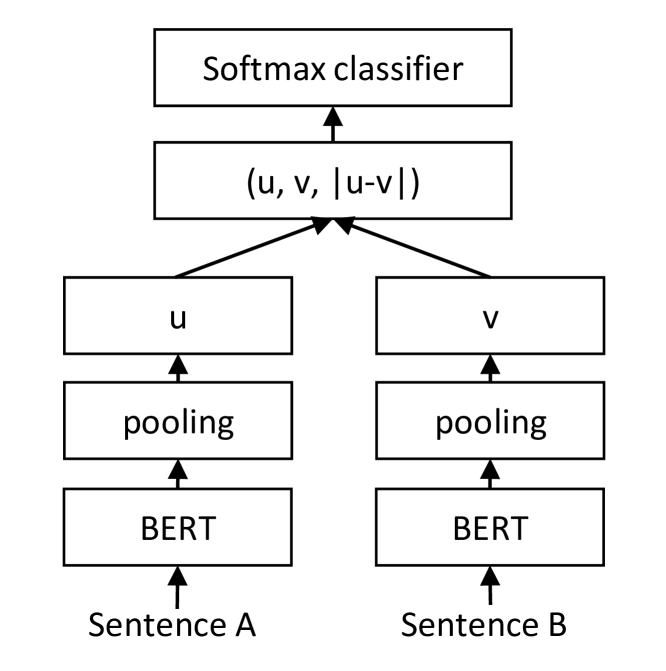
\includegraphics[width=0.60\textwidth]{fig_sbert_biencoder_rgb.png}
\caption{Siamese bi-encoder architecture for dense retrieval, as introduced
  by SBERT~\citep{reimers2019sentence}.  Query and passage are encoded
  independently; relevance is computed as a dot product over the resulting
  vectors.  All dense models evaluated in this study (MiniLM, MPNet, BGE, E5)
  follow this architecture.  Source: \citet{reimers2019sentence} via ar5iv
  (\url{https://arxiv.org/abs/1908.10084}).}
\label{fig:biencoder}
\end{figure}

\paragraph{DPR (Dense Passage Retrieval)~\citep{karpukhin2020dense}.}
Uses \emph{separate} question and context encoders, fine-tuned exclusively on
Natural Questions (NQ) QA pairs.  State-of-the-art on NQ in 2020, but the
narrow training distribution causes catastrophic degradation on out-of-domain
datasets (see Results, Table~\ref{tab:dense}).

\paragraph{BGE and E5 instruction prefixes.}
BGE-base-en-v1.5 prepends \texttt{"Represent this sentence for searching
relevant passages: "} at training time for asymmetric retrieval.
E5-base-v2 uses \texttt{"query: "} / \texttt{"passage: "} prefix tokens to
signal the encoding role.  These instruction-aware models achieve strong
zero-shot performance via large-scale contrastive pre-training with hard
negative mining.

\begin{table}[h]
\centering
\caption{Dense bi-encoder models and their key references.}
\label{tab:dense_model_refs}
\begin{tabular}{lllll}
\toprule
\textbf{Model} & \textbf{Params} & \textbf{Year} & \textbf{Key contribution} & \textbf{ArXiv} \\
\midrule
DPR (question enc.)      & 110M & 2020 & Task-specific dual-encoder on NQ  & 2004.04906 \\
all-MiniLM-L6-v2         & 22M  & 2021 & Distillation from MPNet; 1B pairs  & N/A \\
all-mpnet-base-v2         & 110M & 2021 & Permuted LM + MLM objective        & 2004.09297 \\
BGE-base-en-v1.5          & 110M & 2023 & Hard-neg mining + instruction      & 2309.07597 \\
E5-base-v2                & 110M & 2022 & Weakly-supervised contrastive pre-training & 2212.03533 \\
\bottomrule
\end{tabular}
\end{table}

% -----------------------------------------------------------------------------
\subsection{Model Architecture Details}
% -----------------------------------------------------------------------------

\paragraph{MiniLM: Deep Self-Attention Distillation~\citep{wang2020minilm}.}
\texttt{all-MiniLM-L6-v2} is a 22M-parameter student distilled from a large
MPNet teacher using \emph{self-attention transfer}: the student mimics the
teacher's self-attention distributions and value-relation matrices, not just
the final hidden states.  This makes it 5$\times$ smaller than its teacher
while retaining $>$99\% of retrieval quality on MS MARCO.

\begin{figure}[htbp]
\centering
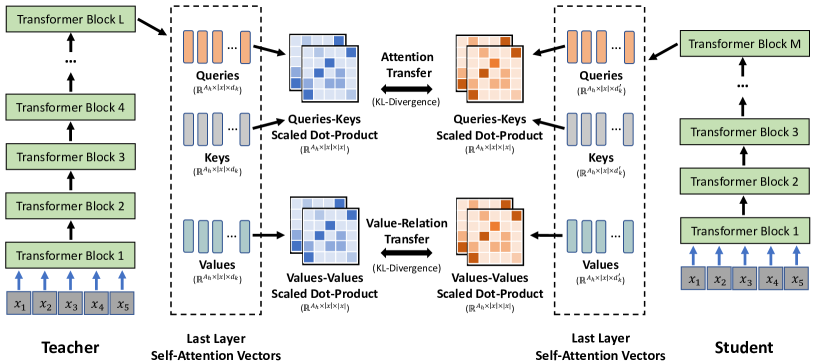
\includegraphics[width=0.78\textwidth]{fig_minilm_arch_rgb.png}
\caption{MiniLM: deep self-attention distillation.  The student mimics the
  teacher's self-attention distributions and value-relation matrices layer by
  layer.  Source: \citet{wang2020minilm} via ar5iv
  (\url{https://arxiv.org/abs/2002.10957}).}
\label{fig:minilm}
\end{figure}

\paragraph{MPNet: Masked and Permuted Language Modelling~\citep{song2020mpnet}.}
BERT's masked LM (MLM) predicts masked tokens but cannot see their positional
context.  XLNet's permuted LM (PLM) uses autoregressive prediction but misses
dependency between predicted tokens.  MPNet combines both: it uses a PLM
objective \emph{with} auxiliary position information from the full sentence,
eliminating the pretrain--finetune discrepancy.

\begin{figure}[htbp]
\centering
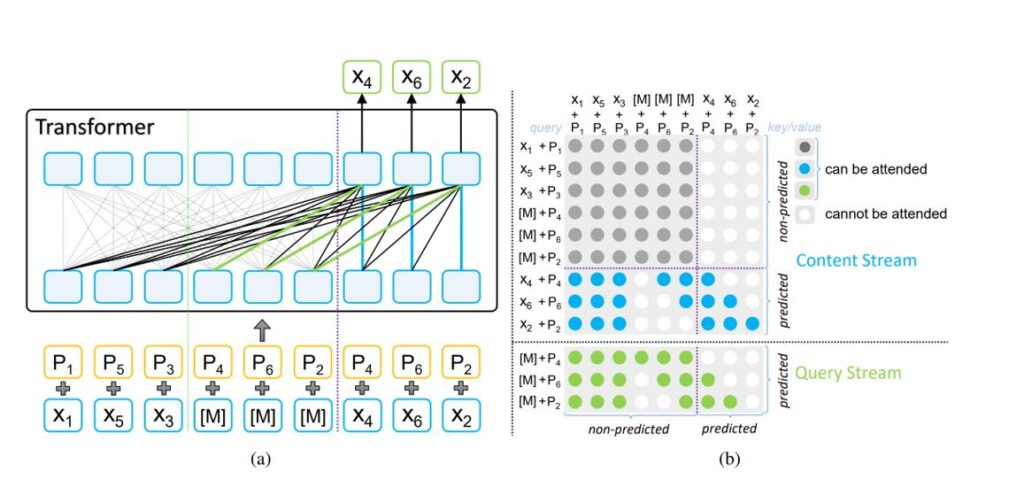
\includegraphics[width=0.82\textwidth]{fig_mpnet_arch.jpg}
\caption{MPNet attention-mask patterns for MLM, PLM, and the combined MPNet
  objective.  Source: \citet{song2020mpnet} via Microsoft Research blog
  (\url{https://www.microsoft.com/en-us/research/blog/mpnet-combines-strengths-of-masked-and-permuted-language-modeling-for-language-understanding/}).}
\label{fig:mpnet}
\end{figure}

\paragraph{E5: Weakly-Supervised Contrastive Pre-training~\citep{wang2022text}.}
E5 curates $\sim$1.3B (text, text$^+$) pairs from web sources (CCPairs) with
consistency filtering.  Stage 1 is large-scale contrastive pre-training with
in-batch negatives on this weakly labelled data.  Stage 2 fine-tunes on
high-quality labelled data (MS MARCO, NLI).  The \texttt{"query: "} /
\texttt{"passage: "} prefix tells the encoder which role to play during
asymmetric retrieval.

\begin{figure}[htbp]
\centering
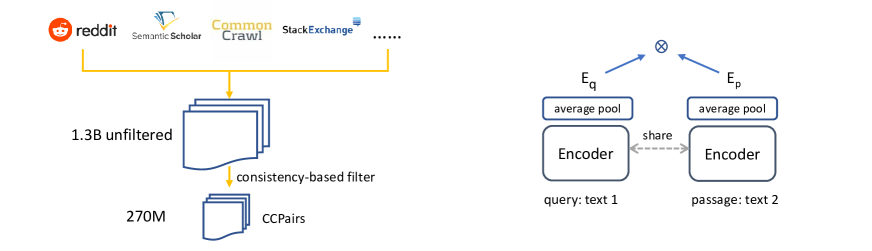
\includegraphics[width=0.80\textwidth]{fig_e5_arch_rgb.png}
\caption{E5 two-stage training pipeline: weakly-supervised contrastive
  pre-training on CCPairs (Stage~1) followed by fine-tuning on labelled data
  (Stage~2).  Source: \citet{wang2022text} via ar5iv
  (\url{https://arxiv.org/abs/2212.03533}).}
\label{fig:e5}
\end{figure}

\paragraph{BGE: Hard-Negative Mining + Instruction Tuning~\citep{xiao2023c}.}
BGE (BAAI General Embedding) trains with a two-step recipe: (1) contrastive
pre-training on large web corpora; (2) fine-tuning with \emph{hard negatives}
mined from an initial retrieval run.  Hard negatives are passages ranked high
by BM25 or a weaker dense model but labelled non-relevant, forcing the
model to learn fine-grained discrimination.  BGE's instruction prefix
(\texttt{"Represent this sentence for searching relevant passages: "})

\begin{figure}[htbp]
\centering
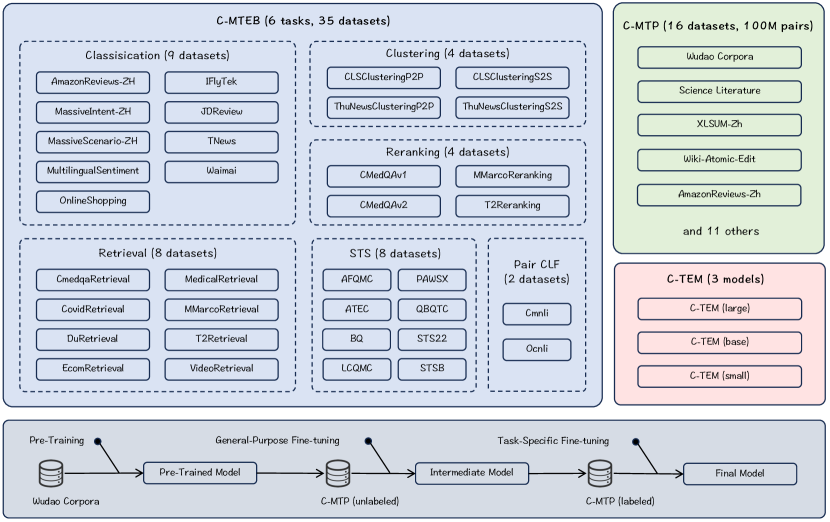
\includegraphics[width=0.80\textwidth]{fig_bge_arch_rgb.png}
\caption{BGE/C-Pack training recipe: large-scale contrastive pre-training
  followed by hard-negative mining and instruction-aware fine-tuning.
  Source: \citet{xiao2023c} via ar5iv
  (\url{https://arxiv.org/abs/2309.07597}).}
\label{fig:bge}
\end{figure}
signals the encoding role for asymmetric retrieval, similar to E5.

% -----------------------------------------------------------------------------
\subsection{Experimental Results}
% -----------------------------------------------------------------------------

\begin{table}[h]
\centering
\caption{Dense retrieval: \ndcg{}.  Bold = best dense model per dataset.
  DPR included as a cautionary baseline.}
\label{tab:dense}
\begin{tabular}{lcccc}
\toprule
\textbf{Model} & \textbf{Params} & \textbf{\tc{}} & \textbf{\fiqa{}} & \textbf{\scifact{}} \\
\midrule
DPR             & 110M & 0.1444 & 0.0601 & 0.2189 \\
MiniLM-L6       & 22M  & 0.4725 & 0.3687 & 0.6451 \\
MPNet-base      & 110M & 0.5133 & \textbf{0.4996} & 0.6557 \\
E5-base         & 110M & 0.6963 & 0.3987 & 0.7194 \\
BGE-base        & 110M & \textbf{0.7807} & 0.4062 & \textbf{0.7404} \\
\midrule
BM25 (reference) & N/A & 0.4471 & 0.1591 & 0.5597 \\
\bottomrule
\end{tabular}
\end{table}

\paragraph{Findings.}
BGE dominates on \tc{} and \scifact{}; instruction-tuned contrastive
training with hard-negative mining gives it a clear edge.  MPNet is the best
model on \fiqa{} despite being older and same-sized as BGE and E5; its
permuted language model objective may better align with conversational
financial queries.  DPR is a cautionary result: NQ-only training collapses
on all three out-of-domain benchmarks, performing below BM25 and even below
Word2Vec on \tc{}.  All general sentence encoders surpass BM25 on all three
datasets; model breadth of training distribution matters more than
domain-specific fine-tuning for zero-shot generalisation.

\paragraph{Illustrative per-query examples.}
\begin{itemize}

\item \textbf{DPR failure (domain shift).}\\
  DPR scores \ndcg{} 0.060 on \fiqa{} and 0.219 on \scifact{} — below BM25
  and even Word2Vec on all three benchmarks.  Trained exclusively on Natural
  Questions (Wikipedia QA), DPR is not architecturally broken; it is the
  narrowest training distribution of any model evaluated and collapses
  completely outside its training domain.

\item \textbf{All dense models solved the OOV problem that Word2Vec could not.}\\
  \textit{Query:} ``ADAR1 binds to Dicer to cleave pre-miRNA.'' (\scifact{})\\
  \textit{Expected passage:} \textit{ADAR1 Forms a Complex with Dicer to Promote
    MicroRNA Processing.} ``ADAR1 forms a complex with Dicer through direct
    protein-protein interaction and increases the maximum rate of pre-miRNA
    cleavage.''\\
  \textit{Why it worked:} All transformer-based models (MiniLM, MPNet, BGE) use
    subword tokenisation, decomposing \texttt{ADAR1} and \texttt{Dicer} into
    known byte-pair units.  All three rank the relevant passage at position~1.
    Word2Vec dropped both identifiers silently as OOV and retrieved an unrelated
    passage.

\item \textbf{BGE succeeded where other dense models struggled (hard-negative training).}\\
  \textit{Query:} ``Ubiquitin ligase UBC13 generates a K63-linked polyubiquitin
    moiety at PCNA K164.'' (\scifact{})\\
  \textit{Expected passage:} \textit{Replication Fork Slowing and Reversal upon
    DNA Damage Require PCNA Polyubiquitination.} ``DNA damage tolerance during
    eukaryotic replication is orchestrated by PCNA ubiquitination; polyubiquitination
    activates an error-free damage bypass pathway.''\\
  \textit{Retrieved (rank 1) by MiniLM and MPNet:} \textit{Evolution and function
    of ubiquitin-like protein-conjugation systems.} (related ubiquitin topic
    but not the specific PCNA K164 pathway; first relevant at ranks 10 and 5
    respectively)\\
  \textit{Why BGE won:} Hard-negative mining during training forces BGE to
    distinguish between passages from the same topic area (ubiquitin biology).
    MiniLM and MPNet, trained without hard negatives, conflate the general
    ubiquitin-pathway passage with the specific PCNA K164 claim.

\item \textbf{Dense models partially failed (clinical specificity bottleneck).}\\
  \textit{Query:} ``p16INK4A accumulation is linked to an abnormal wound response
    caused by the microinvasive step of advanced Oral Potentially Malignant
    Lesions (OPMLs).'' (\scifact{})\\
  \textit{Expected passage:} \textit{Monitoring Tumorigenesis and Senescence In
    Vivo with a p16INK4a-Luciferase Model.}\\
  \textit{Retrieved (rank 1):} MiniLM and BGE retrieve \textit{p16INK4A is a
    robust in vivo biomarker of cellular aging} (related but wrong claim);
    MPNet retrieves \textit{Tumor-associated macrophages correlate with EMT in
    oral squamous cell carcinoma} (shares \texttt{oral} + cancer context).\\
  \textit{Why it partially failed:} MiniLM and BGE retrieve the relevant passage
    within the top-10 (ranks 3 and 4) but not at rank~1; MPNet misses it
    entirely (rank~13, \ndcg{} = 0.000).  The three clinical identifiers
    (\texttt{p16INK4A}, \texttt{microinvasive}, \texttt{OPMLs}) introduce enough
    specificity that even subword tokenisation cannot fully preserve their
    combined meaning in a single fixed-size vector.

\end{itemize}

% =============================================================================
\section{Phase 4: Hybrid Retrieval and Reranking}
\label{sec:hybrid}
% =============================================================================

% -----------------------------------------------------------------------------
\subsection{Why Combine Lexical and Dense Retrieval?}
% -----------------------------------------------------------------------------

Sparse and dense retrievers have complementary strengths and weaknesses:

\begin{itemize}
  \item \textbf{BM25} excels at \emph{exact-match} for rare, discriminative
        terms (acronyms, named entities, product IDs, molecular names).
        It fails when the query and relevant passage use different vocabulary
        (synonym gap).
  \item \textbf{Dense models} excel at \emph{semantic matching}; they
        retrieve passages that are conceptually similar even with zero term
        overlap.  They can struggle with very specific rare terms that were
        unseen or rare in pre-training.
\end{itemize}

RRF fusion (Equation~\ref{eq:rrf}, $k=60$) combines both ranked lists
without requiring a trained combiner, making it parameter-free and robust.
The $k=60$ default prevents a single high-rank appearance in one list from
dominating the fused score.

% -----------------------------------------------------------------------------
\subsection{System Architecture}
% -----------------------------------------------------------------------------

\begin{figure}[h]
\centering
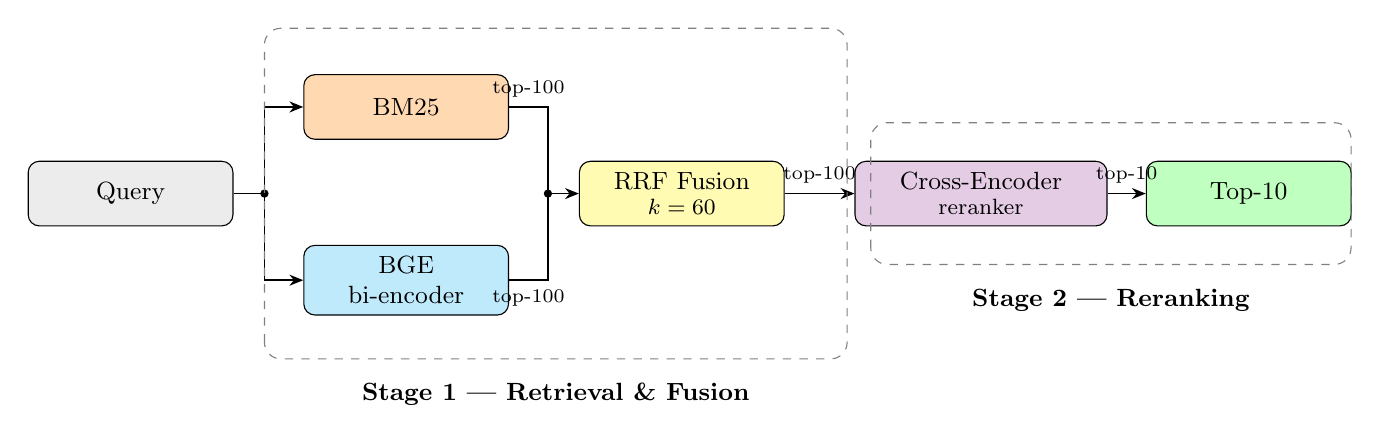
\begin{tikzpicture}[
  box/.style={draw, rounded corners=4pt, minimum width=2.6cm, minimum height=0.82cm,
              align=center, font=\small, inner sep=4pt},
  arr/.style={-{Stealth[length=5pt,width=4pt]}, semithick},
  lin/.style={semithick},
  slbl/.style={font=\scriptsize}
]

%% Nodes
\node[box, fill=gray!15]   (q)    at (0.0,  0)    {Query};
\node[box, fill=orange!30] (bm25) at (3.5,  1.1)  {BM25};
\node[box, fill=cyan!25]   (bge)  at (3.5, -1.1)  {BGE\\bi-encoder};
\node[box, fill=yellow!30] (rrf)  at (7.0,  0)    {RRF Fusion\\[-2pt]{\footnotesize $k=60$}};
\node[box, fill=violet!20, minimum width=3.2cm]
                           (ce)   at (10.8, 0)    {Cross-Encoder\\[-2pt]{\footnotesize reranker}};
\node[box, fill=green!25]  (out)  at (14.2, 0)    {Top-10};

%% Fork point (Query -> retrievers)
\coordinate (fork) at (1.7, 0);
\draw[lin] (q.east) -- (fork);
\draw[arr] (fork) |- (bm25.west);
\draw[arr] (fork) |- (bge.west);
\fill (fork) circle (1.5pt);

%% Merge point (retrievers -> RRF): one arrowhead into RRF
\coordinate (merge) at (5.3, 0);
\draw[lin] (bm25.east) -- node[slbl, above] {top-100} (merge |- bm25.east) -- (merge);
\draw[lin] (bge.east)  -- node[slbl, below] {top-100} (merge |- bge.east)  -- (merge);
\draw[arr] (merge) -- (rrf.west);
\fill (merge) circle (1.5pt);

%% RRF -> Cross-Encoder -> Output
\draw[arr] (rrf.east) -- node[slbl, above] {top-100} (ce.west);
\draw[arr] (ce.east)  -- node[slbl, above] {top-10}  (out.west);

%% Stage annotation boxes
\draw[dashed, gray, rounded corners=6pt]
  (1.7, -2.1) rectangle (9.1, 2.1);
\node[font=\small\bfseries] at (5.4, -2.55)
  {Stage~1 --- Retrieval \& Fusion};

\draw[dashed, gray, rounded corners=6pt]
  (9.4, -0.90) rectangle (15.5, 0.90);
\node[font=\small\bfseries] at (12.45, -1.35)
  {Stage~2 --- Reranking};

\end{tikzpicture}
\caption{Two-stage hybrid retrieval pipeline.
  \textbf{Stage~1 (Retrieval \& Fusion):} BM25 and BGE independently retrieve
  the top-100 candidates; their ranked lists are merged via Reciprocal Rank
  Fusion ($k=60$) into a unified top-100 candidate set.
  \textbf{Stage~2 (Reranking):} a cross-encoder
  (\texttt{ms-marco-MiniLM-L-6-v2}) scores every (query, passage) pair in
  the candidate set and returns the final top-10.}
\label{fig:pipeline}
\end{figure}

\begin{enumerate}
  \item BM25 and BGE independently retrieve top-100 candidates.
  \item Scores are fused via RRF (Equation~\ref{eq:rrf}, $k=60$).
  \item A cross-encoder (\texttt{cross-encoder/ms-marco-MiniLM-L-6-v2})
        reranks the top-100 RRF candidates.
  \item Top-10 are returned for evaluation.
\end{enumerate}

\paragraph{Cross-encoder vs.\ bi-encoder.}
The cross-encoder processes the concatenated sequence
$[\text{CLS}]\; q\; [\text{SEP}]\; p\; [\text{SEP}]$ through a single
transformer, allowing every query token to attend to every passage token:
\begin{equation}
  \text{score}_{\text{CE}}(q, p)
    = \text{Linear}\!\left(\text{BERT}([\text{CLS}]\; q\; [\text{SEP}]\; p)_{[\text{CLS}]}\right)
    \in \mathbb{R}
  \label{eq:cross_encoder}
\end{equation}
This \emph{full interaction} produces more accurate relevance scores than a
dot product over independent vectors.  The trade-off: passage embeddings
cannot be pre-computed, so inference cost is $O(|Q| \times |\text{candidates}|)$,
making it practical only for reranking a small candidate set (top-100).

% -----------------------------------------------------------------------------
\subsection{Experimental Results}
% -----------------------------------------------------------------------------

\begin{table}[h]
\centering
\caption{Hybrid retrieval: \ndcg{}.  Bold = best overall per dataset.}
\label{tab:hybrid_ndcg}
\begin{tabular}{lccc}
\toprule
\textbf{Method} & \textbf{\tc{}} & \textbf{\fiqa{}} & \textbf{\scifact{}} \\
\midrule
BM25 (sparse)        & 0.4471 & 0.1591 & 0.5597 \\
BGE (best dense)     & \textbf{0.7807} & \textbf{0.4062} & \textbf{0.7404} \\
Hybrid RRF           & 0.7100 & 0.2921 & 0.6674 \\
Hybrid + Reranker    & 0.7630 & 0.3743 & 0.6888 \\
\bottomrule
\end{tabular}
\end{table}

\begin{table}[h]
\centering
\caption{Recall and MAP for hybrid methods across all datasets.}
\label{tab:hybrid_recall}
\begin{tabular}{lcccc}
\toprule
\textbf{Method} & \textbf{\map{}} & \textbf{Recall@10} & \textbf{Recall@50} & \textbf{Recall@100} \\
\midrule
\multicolumn{5}{l}{\textit{\fiqa{}}} \\
Hybrid RRF           & 0.2423 & 0.3690 & 0.6255 & 0.6964 \\
Hybrid + Reranker    & 0.3119 & 0.4574 & 0.6334 & 0.6965 \\
\midrule
\multicolumn{5}{l}{\textit{\scifact{}}} \\
Hybrid RRF           & 0.6296 & 0.7977 & 0.9343 & 0.9527 \\
Hybrid + Reranker    & \textbf{0.6520} & \textbf{0.8089} & 0.9303 & 0.9527 \\
\midrule
\multicolumn{5}{l}{\textit{\tc{}}} \\
Hybrid RRF           & 0.0830 & 0.0189 & 0.0723 & 0.1197 \\
Hybrid + Reranker    & 0.0932 & 0.0209 & 0.0837 & 0.1195 \\
\bottomrule
\end{tabular}
\end{table}

\paragraph{Findings.}
Counter to the common assumption that hybrid always beats dense,
\textbf{BGE alone outperforms Hybrid+Reranker} on both \tc{} (0.781
vs.\ 0.763) and \fiqa{} (0.406 vs.\ 0.374).  The culprit is BM25:
when the sparse component is weak (conversational queries on \fiqa{};
highly specialised biomedical vocabulary on \tc{}), RRF fusion
\emph{degrades} the dense signal.  Adding the cross-encoder reranker
partially recovers this loss (+0.05 on \tc{}, +0.08 on \fiqa{}), but
does not reach BGE alone on \tc{}.

The reranker does not improve Recall@100; it only reorders the same
100 candidates, and Recall@100 matches exactly for RRF vs.\ Reranker.
The reranker's value is better precision at small $k$: Recall@10 improves
by +0.088 on \fiqa{} and +0.011 on \scifact{}.

\paragraph{Illustrative per-query examples.}
\begin{itemize}
  \item \textbf{RRF hurt on \scifact{}.}  BGE alone achieves Recall@100 = 0.967
        on \scifact{}, already covering 96.7\% of relevant passages.
        Equal-weight RRF allows BM25's top-ranked (often incorrect) passages
        to displace BGE's lower-ranked but still relevant ones, reducing
        \ndcg{} from 0.740 to 0.667 ($-0.073$).  When one retriever dominates,
        equal-weight fusion dilutes rather than complements.
  \item \textbf{Cross-encoder recovered precision on \fiqa{}.}  The reranker
        improves Recall@10 from 0.369 to 0.457 (+8.8 pp) by jointly encoding
        each (query, passage) pair.  A bi-encoder dot product scores query
        and passage independently, so it can miss fine-grained distinctions
        between passages that share surface vocabulary but address different
        questions.  The cross-encoder attends across both texts simultaneously,
        providing a more accurate relevance signal within the re-ranked shortlist.
\end{itemize}

% =============================================================================
\section{Extension A: Domain-Specific Fine-tuning}
\label{sec:finetune}
% =============================================================================

\subsection{Setup}

We fine-tune \texttt{all-MiniLM-L6-v2} (22M parameters) using
MultipleNegativesRankingLoss (Equation~\ref{eq:mnr}).  Training pairs are
constructed from BEIR qrels: each (query, positive passage) pair from the
training split.  Three fine-tuning variants are evaluated.

\begin{table}[h]
\centering
\caption{Fine-tuning experimental variants.}
\label{tab:ft_setup}
\begin{tabular}{lrrl}
\toprule
\textbf{Variant} & \textbf{Train pairs} & \textbf{Time} & \textbf{Epochs} \\
\midrule
ft-\fiqa{}      & 14,131 & 6.3 min & 3 \\
ft-\scifact{}   & 919    & 1.1 min & 5 \\
ft-Combined     & 15,050 & 6.7 min & 3 \\
\bottomrule
\end{tabular}
\end{table}

\subsection{Experimental Results}

\begin{table}[h]
\centering
\caption{Fine-tuning results: \ndcg{}.  Base model = \texttt{all-MiniLM-L6-v2}.
  Bold = improvement over base.}
\label{tab:finetune}
\begin{tabular}{lcccc}
\toprule
\textbf{Model} & \textbf{Train pairs} & \textbf{\tc{}} & \textbf{\fiqa{}} & \textbf{\scifact{}} \\
\midrule
MiniLM base        & N/A    & 0.4725 & 0.3687 & 0.6451 \\
ft-\fiqa{}         & 14,131 & \textbf{0.4867} & \textbf{0.3964} & 0.6451 \\
ft-\scifact{}      & 919    & 0.4606 & 0.3593 & \textbf{0.6949} \\
ft-Combined        & 15,050 & \textbf{0.5027} & \textbf{0.3997} & \textbf{0.6596} \\
\bottomrule
\end{tabular}
\end{table}

\begin{table}[h]
\centering
\caption{Primary: in-domain gain.  Each variant is judged on the
  dataset(s) it was trained on.}
\label{tab:ft_delta_indomain}
\begin{tabular}{llcc}
\toprule
\textbf{Fine-tuned on} & \textbf{Eval dataset} & \textbf{Base \ndcg{}} & \textbf{$\Delta$} \\
\midrule
\scifact{}            & \scifact{}  & 0.6451 & $+0.0498$ \\
\fiqa{}               & \fiqa{}     & 0.3687 & $+0.0277$ \\
Combined              & \scifact{}  & 0.6451 & $+0.0145$ \\
Combined              & \fiqa{}     & 0.3687 & $+0.0310$ \\
\bottomrule
\end{tabular}
\end{table}

\begin{table}[h]
\centering
\caption{Secondary: cross-domain impact (catastrophic forgetting check).
  Eval dataset was \emph{not} in the training set.}
\label{tab:ft_delta_crossdomain}
\begin{tabular}{llcc}
\toprule
\textbf{Fine-tuned on} & \textbf{Eval dataset} & \textbf{Base \ndcg{}} & \textbf{$\Delta$} \\
\midrule
\scifact{}     & \fiqa{}  & 0.3687 & $-0.0094$ \\
\scifact{}     & \tc{}    & 0.4725 & $-0.0119$ \\
\fiqa{}        & \scifact{} & 0.6451 & $0.0000$ \\
\fiqa{}        & \tc{}    & 0.4725 & $+0.0142$ \\
Combined       & \tc{}    & 0.4725 & $+0.0302$ \\
\bottomrule
\end{tabular}
\end{table}

\paragraph{Findings.}
\begin{itemize}
  \item \textbf{In-domain specialisation is strong and data-efficient
        (Table~\ref{tab:ft_delta_indomain}).}
        Fine-tuning on 919 SciFact pairs (+7.7\%) achieves comparable
        relative gain to 14,131 FIQA pairs (+7.5\%).  Recall@10 on
        \scifact{} jumps from 0.783 to 0.865 (+8.2 percentage points).

  \item \textbf{Negative transfer is real but small
        (Table~\ref{tab:ft_delta_crossdomain}).}
        \scifact{} fine-tuning hurts \fiqa{} ($-0.009$) and \tc{} ($-0.012$);
        domain specialisation trades breadth for depth.  The penalty is
        modest compared to the in-domain gain.

  \item \textbf{Combined training generalises to unseen domains.}
        ft-Combined is the only variant that improves all three datasets
        simultaneously, including \tc{} (+3.0\%) which appears in neither
        training set.  \tc{} has no training split in BEIR; ft-Combined
        is the closest proxy available, and its cross-domain transfer
        demonstrates that multi-domain training reduces specialisation cost.

  \item \textbf{Small model + in-domain data beats larger zero-shot models.}
        ft-\scifact{} MiniLM (22M, NDCG 0.695) exceeds MPNet (110M, 0.656)
        and approaches E5 (110M, 0.719) on \scifact{}, with 5$\times$ fewer
        parameters with targeted data.
\end{itemize}

\paragraph{Embedding-space effect.}
Before fine-tuning, base MiniLM assigns irrelevant pairs a mean cosine
similarity of $0.089$ — uncomfortably close to the relevant-pair mean of
$0.586$.  After fine-tuning on \scifact{}, irrelevant-pair similarity drops to
$0.026$ while the relevant-pair mean holds at $0.573$.  The separation gap
widens from $0.497$ to $0.547$: the gain does not come from pulling relevant
passages closer, but from pushing irrelevant ones further away.  This directly
explains the $+7.7\%$ NDCG improvement.

\paragraph{Illustrative per-query improvement.}
\begin{itemize}
  \item \textbf{Domain-specific claim matched after fine-tuning.}
        \textit{Query:} ``The PPR MDA5 has two N-terminal CARD domains.''
        \textit{Expected passage (title):} ``Immune signaling by RIG-I-like receptors.''\\
        \textit{Base MiniLM (rank 161):} Returns ``Chaperoning 5S RNA assembly'' — a
        ribosomal RNA paper with no connection to innate immunity. The base model has
        no representation of \textit{MDA5} (a pattern recognition receptor) or
        \textit{CARD domains} in the antiviral signalling context, so it makes an
        arbitrary match on surface-level RNA co-occurrence.\\
        \textit{Fine-tuned MiniLM (rank 2):} The model trained on SciFact
        biomedical claim–evidence pairs learns that claims about specific protein
        domain architecture (CARD, DEAD-box helicase) belong in the innate immunity
        literature.  The correct review of RIG-I-like receptors — which explicitly
        covers MDA5 domain structure — advances from rank~161 to rank~2.
\end{itemize}

% =============================================================================
\section{Note on LLM-as-Judge Evaluation}
\label{sec:llm_judge}
% =============================================================================

Standard IR evaluation relies on manually curated qrels.  For all experiments
in this study, NDCG and MRR are the right metrics: the BEIR benchmarks provide
high-quality human relevance judgements, and qrel-based metrics are
reproducible, fast, and interpretable.

LLM-as-judge evaluation (prompting a language model to score each retrieved
passage for relevance) is a separate technique warranting consideration in
the following scenarios.

\paragraph{When LLM-as-judge adds value.}
\begin{itemize}
  \item \textbf{No ground-truth labels.}  For a private corpus or a domain
        not covered by existing benchmarks, there are no qrels.  An LLM
        judge provides the only automated relevance signal without costly
        human annotation.
  \item \textbf{Sparse qrel coverage (annotation gaps).}  Benchmark qrels
        are constructed by pooling candidates from a baseline retriever.  A
        stronger model may surface genuinely relevant passages that were never
        judged; these appear as false positives in NDCG even when they are
        correct.  An LLM judge can identify such cases.
  \item \textbf{End-to-end RAG evaluation.}  Once a generator is in the
        pipeline, the question shifts from ``did the right chunk rank first?''
        to ``did the generated answer use the retrieved evidence correctly?''
        Metrics such as faithfulness and answer relevancy require an LLM
        to assess; there is no qrel-based equivalent.
  \item \textbf{Fine-tuned model on held-out queries without annotated qrels.}
        If the deployment domain has no labelled test split, an LLM judge
        provides a directional signal for measuring improvement.
\end{itemize}

\paragraph{Key caveats.}
\begin{itemize}
  \item \textbf{The judge must be capable for the domain.}  A small model
        (e.g.\ 3B parameters) judging specialised scientific claims will
        produce unreliable scores , not because the technique is broken, but because the model lacks the domain knowledge to assess relevance
        accurately.  For specialist domains, a larger or domain-adapted judge
        is required.
  \item \textbf{Scores are not comparable across judge models.}  Absolute
        context-precision values are specific to the judge setup; only
        relative comparisons within the same configuration are meaningful.
  \item \textbf{Cost scales with queries $\times$ candidates.}  Each
        (query, passage) pair requires one LLM call.  Sample 100--200
        queries for a directional signal rather than scoring the full set.
\end{itemize}

For the retrieval paradigms studied here (sparse, dense, hybrid, and
fine-tuned bi-encoders on established BEIR benchmarks), NDCG@10 is
the appropriate primary metric throughout.

% =============================================================================
\section{Discussion}
\label{sec:discussion}
% =============================================================================

\subsection{When Does Hybrid Retrieval Help?}

Hybrid RRF improves over both components only when both are competitive.
When BM25 is systematically weak (conversational or highly domain-specific
queries), it introduces noise into the fusion and RRF can \emph{hurt} dense
retrieval.  The cross-encoder reranker is a more robust upgrade: it acts on
the candidate set regardless of how it was assembled, and consistently yields
+0.02--0.08 NDCG across all datasets.

\textbf{Practical implication:} for production RAG systems, prefer
dense-only + cross-encoder over BM25+dense hybrid unless BM25 quality
on the target domain is validated first.

\subsection{Fine-tuning Efficiency vs.\ Scale}

The \scifact{} experiment demonstrates that \emph{very few} high-quality
training pairs suffice for significant improvement (919 pairs, 1.1 min on
Apple M5 MPS).  The key mechanism is MNR loss's in-batch negatives: with
batch size 64, each positive pair is contrasted against 63 negatives per
step without requiring hard-negative mining.

\subsection{When to Move Beyond NDCG}

NDCG is the right metric when high-quality qrels exist, as in all three
benchmarks used here.  The main scenario where it falls short is
\emph{annotation gap}: a better model retrieves genuinely relevant
passages that pooling-based annotation never assessed, and NDCG penalises
them as false positives.

For production systems without labelled data, LLM-as-judge provides a
directional signal, but the judge must match the domain.  A small general
model judging scientific claims or biomedical queries will apply generic
topical relevance rather than the task-specific relevance criteria that the
qrels encode.  The practical implication: use a capable, domain-appropriate
judge, treat scores as relative rather than absolute, and reserve the
technique for the scenarios listed in Section~\ref{sec:llm_judge}.

% =============================================================================
\section{Conclusion}
\label{sec:conclusion}
% =============================================================================

We have traced the evolution of information retrieval across four paradigms,
from BoW to fine-tuned neural encoders, on three heterogeneous BEIR benchmarks.
Key takeaways:

\begin{enumerate}
  \item BM25 is a strong, zero-cost baseline but \emph{not always the best
        sparse method}: TF-IDF's implicit global normalisation outperforms
        BM25 on short, uniform corpora (\scifact{}, \fiqa{}).
  \item Dense bi-encoders with general contrastive training (BGE, E5) beat
        BM25 across all three datasets.  Task-specific fine-tuning (DPR)
        without data diversity produces brittle, domain-fragile models,
        performing below BM25 and Word2Vec on out-of-domain benchmarks.
  \item Hybrid RRF is not universally better than dense retrieval; it
        requires a competitive sparse component.  The cross-encoder reranker
        is a more reliable upgrade (+0.02--0.08 NDCG across all settings).
  \item Domain-specific fine-tuning with MNR loss is highly data-efficient;
        919 \scifact{} pairs deliver +7.7\% in-domain NDCG with under
        2 minutes of training on consumer hardware.  Combined multi-domain
        training generalises to unseen domains without negative transfer.
  \item LLM-as-judge is not appropriate as a primary metric when
        annotated qrels exist.  Its value is in evaluating private corpora
        with no labels, surfacing annotation gaps in large benchmarks, and
        assessing end-to-end RAG quality beyond rank-based metrics.
\end{enumerate}

% =============================================================================
\section*{Acknowledgements}
% =============================================================================
% Placeholder: add institutional acknowledgements here.

% =============================================================================
\section*{Code and Data}
% =============================================================================

The full source for this study is available at\\
\url{https://github.com/saikrishnab-sahajai/retrieval-evolution-study}.\\
The repository includes all evaluation scripts, result files (JSON), and
notebooks.  Large corpus files and fine-tuned model checkpoints are excluded
but can be reproduced via \texttt{scripts/download\_datasets.py} and
\texttt{scripts/run\_finetune.py}.

% =============================================================================
% Bibliography
% =============================================================================
\begin{thebibliography}{99}

\bibitem[Cormack et~al.(2009)]{cormack2009reciprocal}
Cormack, G.~V., Clarke, C.~L.~A., and Buettcher, S. (2009).
Reciprocal rank fusion outperforms Condorcet and individual rank learning
methods.
\textit{SIGIR '09}.

\bibitem[Devlin et~al.(2019)]{devlin2019bert}
Devlin, J., Chang, M.-W., Lee, K., and Toutanova, K. (2019).
BERT: Pre-training of deep bidirectional transformers for language
understanding.
\textit{NAACL-HLT}.

\bibitem[Hadsell et~al.(2006)]{hadsell2006dimensionality}
Hadsell, R., Chopra, S., and LeCun, Y. (2006).
Dimensionality reduction by learning an invariant mapping.
\textit{CVPR}.

\bibitem[Henderson et~al.(2017)]{henderson2017efficient}
Henderson, M., Al-Rfou, R., Strope, B., et~al. (2017).
Efficient natural language response suggestion for smart reply.
\textit{arXiv:1705.00652}.

\bibitem[Karpukhin et~al.(2020)]{karpukhin2020dense}
Karpukhin, V., O\u{g}uz, B., Min, S., Lewis, P., Wu, L., Edunov, S.,
Chen, D., and Yih, W.-t. (2020).
Dense passage retrieval for open-domain question answering.
\textit{EMNLP}. \url{https://arxiv.org/abs/2004.04906}.

\bibitem[Khattab and Zaharia(2020)]{khattab2020colbert}
Khattab, O. and Zaharia, M. (2020).
ColBERT: Efficient and effective passage search via contextualized late
interaction over BERT.
\textit{SIGIR}. \url{https://arxiv.org/abs/2004.12832}.

\bibitem[Wang et~al.(2020)]{wang2020minilm}
Wang, W., Wei, F., Dong, L., Bao, H., Yang, N., and Zhou, M. (2020).
MiniLM: Deep self-attention distillation for task-agnostic compression of
pre-trained transformers.
\textit{NeurIPS}. \url{https://arxiv.org/abs/2002.10957}.

\bibitem[Mikolov et~al.(2013)]{mikolov2013distributed}
Mikolov, T., Sutskever, I., Chen, K., Corrado, G., and Dean, J. (2013).
Distributed representations of words and phrases and their compositionality.
\textit{NeurIPS}. \url{https://arxiv.org/abs/1301.3781}.

\bibitem[Bojanowski et~al.(2017)]{bojanowski2017enriching}
Bojanowski, P., Grave, E., Joulin, A., and Mikolov, T. (2017).
Enriching word vectors with subword information.
\textit{TACL}, 5:135--146. \url{https://arxiv.org/abs/1607.04606}.

\bibitem[Le and Mikolov(2014)]{le2014distributed}
Le, Q. and Mikolov, T. (2014).
Distributed representations of sentences and documents.
\textit{ICML}. \url{https://arxiv.org/abs/1405.4053}.

\bibitem[Pennington et~al.(2014)]{pennington2014glove}
Pennington, J., Socher, R., and Manning, C.~D. (2014).
Glo{V}e: Global vectors for word representation.
\textit{Proceedings of EMNLP}, pages 1532--1543.
\url{https://aclanthology.org/D14-1162}.

\bibitem[Reimers and Gurevych(2019)]{reimers2019sentence}
Reimers, N. and Gurevych, I. (2019).
Sentence-BERT: Sentence embeddings using siamese BERT-networks.
\textit{EMNLP-IJCNLP}. \url{https://arxiv.org/abs/1908.10084}.

\bibitem[Robertson et~al.(1994)]{robertson1994simple}
Robertson, S., Walker, S., Jones, S., Hancock-Beaulieu, M., and Gatford, M. (1994).
Okapi at TREC-3.
\textit{Proceedings of the Third Text REtrieval Conference (TREC-3)}, NIST.

\bibitem[Robertson and Zaragoza(2009)]{robertson2009probabilistic}
Robertson, S. and Zaragoza, H. (2009).
The probabilistic relevance framework: BM25 and beyond.
\textit{Foundations and Trends in Information Retrieval}.

\bibitem[Schroff et~al.(2015)]{schroff2015facenet}
Schroff, F., Kalenichenko, D., and Philbin, J. (2015).
FaceNet: A unified embedding for face recognition and clustering.
\textit{CVPR}.

\bibitem[Song et~al.(2020)]{song2020mpnet}
Song, K., Tan, X., Qin, T., Lu, J., and Liu, T.-Y. (2020).
MPNet: Masked and permuted pre-training for language understanding.
\textit{NeurIPS}. \url{https://arxiv.org/abs/2004.09297}.

\bibitem[Thakur et~al.(2021)]{thakur2021beir}
Thakur, N., Reimers, N., R\"{u}ckl\'{e}, A., Srivastava, A., and
Gurevych, I. (2021).
BEIR: A heterogeneous benchmark for zero-shot evaluation of information
retrieval models.
\textit{NeurIPS Datasets and Benchmarks}.

\bibitem[Wang et~al.(2022)]{wang2022text}
Wang, L., Yang, N., Huang, X., Jiao, B., Yang, L., Jiang, D., Majumder, R.,
and Wei, F. (2022).
Text embeddings by weakly-supervised contrastive pre-training.
\textit{arXiv:2212.03533}.

\bibitem[Xiao et~al.(2023)]{xiao2023c}
Xiao, S., Liu, Z., Zhang, P., and Muennighoff, N. (2023).
C-Pack: Packaged resources to advance general Chinese embedding.
\textit{arXiv:2309.07597}.

\end{thebibliography}

% =============================================================================
\appendix
% =============================================================================

\section{Complete Metric Tables}
\label{app:full_tables}

\begin{table}[h]
\centering
\caption{Full sparse retrieval metrics.}
\label{tab:sparse_full}
\begin{tabular}{llcccc}
\toprule
\textbf{Dataset} & \textbf{Method} & \textbf{\ndcg{}} & \textbf{\mrr{}} & \textbf{\map{}} & \textbf{Recall@10} \\
\midrule
\multirow{3}{*}{\tc{}}
  & BoW    & 0.1763 & 0.3177 & 0.0084 & 0.0035 \\
  & TF-IDF & 0.2866 & 0.5025 & 0.0264 & 0.0077 \\
  & BM25   & 0.4471 & 0.7197 & 0.0413 & 0.0113 \\
\midrule
\multirow{3}{*}{\fiqa{}}
  & BoW    & 0.0656 & 0.0889 & 0.0524 & 0.0791 \\
  & TF-IDF & 0.1793 & 0.2156 & 0.1412 & 0.2435 \\
  & BM25   & 0.1591 & 0.1985 & 0.1239 & 0.2037 \\
\midrule
\multirow{3}{*}{\scifact{}}
  & BoW    & 0.3647 & 0.3424 & 0.3394 & 0.4617 \\
  & TF-IDF & 0.6286 & 0.5897 & 0.5827 & 0.7735 \\
  & BM25   & 0.5597 & 0.5242 & 0.5202 & 0.6862 \\
\bottomrule
\end{tabular}
\end{table}

\begin{table}[h]
\centering
\caption{Full dense retrieval metrics (\ndcg{}, \mrr{}, and Recall@10).}
\label{tab:dense_full}
\begin{tabular}{llccc}
\toprule
\textbf{Dataset} & \textbf{Model} & \textbf{\ndcg{}} & \textbf{\mrr{}} & \textbf{Recall@10} \\
\midrule
\multirow{4}{*}{\tc{}}
  & MiniLM  & 0.4725 & 0.7275 & 0.0128 \\
  & MPNet   & 0.5133 & 0.7576 & 0.0147 \\
  & E5      & 0.6963 & 0.9133 & 0.0196 \\
  & BGE     & 0.7807 & 0.9180 & 0.0221 \\
\midrule
\multirow{4}{*}{\fiqa{}}
  & MiniLM  & 0.3687 & 0.4543 & 0.4413 \\
  & MPNet   & 0.4996 & 0.5886 & 0.5811 \\
  & E5      & 0.3987 & 0.4862 & 0.4705 \\
  & BGE     & 0.4062 & 0.4931 & 0.4814 \\
\midrule
\multirow{4}{*}{\scifact{}}
  & MiniLM  & 0.6451 & 0.6110 & 0.7833 \\
  & MPNet   & 0.6557 & 0.6237 & 0.7901 \\
  & E5      & 0.7194 & 0.6880 & 0.8465 \\
  & BGE     & 0.7404 & 0.7071 & 0.8742 \\
\bottomrule
\end{tabular}
\end{table}

\end{document}
